\documentclass[11pt]{article}
\usepackage[margin=1.1in]{geometry}
\usepackage{booktabs, graphicx, amsmath, natbib, xcolor, hyperref}
\usepackage[T1]{fontenc}
\hypersetup{colorlinks=true, allcolors=blue!60!black}
\title{Does machine learning make loan-loss provisions more volatile?\\
\large Loan-level evidence from 16,000 commercial mortgages}
\author{Eleni Kalamara\thanks{Draft. Code and data pipeline: \texttt{ifrs9\_procyclicality}.}}
\date{\today}

\begin{document}
\maketitle

\begin{abstract}
Supervisors have asked whether machine learning will make regulatory credit measures less stable over the cycle,
on the argument that flexible estimators introduce point-in-time behaviour \citep{eba2021ml}. We test this directly. Using the full public record
of asset-level filings for US conduit commercial mortgage-backed securities, 375 deals and 16{,}437 loans reported
monthly from 2016 to 2026, we build three probability-of-default models that differ only in functional form and in
whether they condition on macroeconomic data, hold loss given default and exposure identical across them, and
compute IFRS 9 and CECL provisions for each. Over an evaluation window fixed in advance by a training-data rule,
provisions built on gradient boosting rise \emph{less} over the commercial real estate downturn than those built
on a logit with the same macro inputs, by $0.26$ of the trough level (95\% interval $0.09$ to $0.44$). The
difference that matters is macroeconomic conditioning, not model flexibility: the point-in-time logit raises
amplitude by $0.85$ relative to a through-the-cycle logit, and its provisions turn eight months before realised
delinquency, while the through-the-cycle model does not lead at all. Stage migration, rather than movement in
probabilities within a stage, accounts for 43 to 81 per cent of the swing in every model. The result is specific
to prime US commercial mortgages and to one downturn, and it does not transfer to corporate or retail portfolios.
\end{abstract}

\section{Introduction}
\label{sec:intro}
IFRS 9 replaced incurred losses with expected losses, and in doing so made provisions forward looking. The
standard was designed to correct the ``too little, too late'' recognition of credit losses that the incurred loss
approach produced \citep{esrb2017ifrs9}. It also introduced two features that make provisions move with the cycle:
credit risk parameters that respond to current conditions, and a staging architecture in which exposures whose
credit risk has increased significantly jump from twelve-month to lifetime loss recognition. The European Systemic
Risk Board identified both channels at the outset, noting that IFRS 9 ``could have certain procyclical effects
derived from the cyclical sensitivity of the credit risk parameters used for the estimation of ECLs and from the
shifts of exposures between stages'' \citep{esrb2017ifrs9}.

A separate concern has grown alongside the first. As banks replace scorecards with machine learning, supervisors
have asked whether more flexible estimators will make regulatory measures less stable over the cycle. The European
Banking Authority put the mechanism plainly in its discussion paper on machine learning for internal models:
machine learning algorithms ``may introduce point-in-time (PiT) elements in the models that may hamper the
stability of the rating assignment process compared to more through-the-cycle (TtC) models leading to potential
rapid changes in capital requirements'' \citep{eba2021ml}. The follow-up report retained the emphasis on
validation and explainability \citep{eba2023ml}, and the European Central Bank has since added a section on
machine learning to its guide to internal models, requiring that such models be ``adequately explainable'' and
that ``their performance justifies their complexity'' \citep{ecb2025guide}.

The mechanism in that sentence bundles two things that can be separated: whether a model conditions on
point-in-time information, and whether it is estimated by a flexible algorithm. A gradient boosting model given no
macroeconomic inputs is not point-in-time; a logistic regression given real-time unemployment is. If the concern
is really about point-in-time behaviour, then it is a concern about an information set that IFRS 9 requires banks
to use, and the estimator is incidental.

This paper separates the two. Using the full public record of asset-level filings for US conduit commercial
mortgage-backed securities, we estimate three probability-of-default models that differ only in functional form
and information set, hold loss given default, exposure and the staging rules identical across them, and compute
IFRS 9 and CECL provisions from each. The design makes the comparison a controlled one: the same loans, the same
months, the same loss rates, and the same threshold for moving between stages.

Three findings follow. First, machine learning does not amplify provisions. Given the same information as the
logit, gradient boosting produces a smaller rise in provisions over the downturn, by $0.26$ of the trough level
(interval $-0.44$ to $-0.09$), and the sign survives every robustness specification we ran. Second, point-in-time
conditioning does amplify them: replacing the through-the-cycle logit with a point-in-time logit raises amplitude
by $0.85$. Third, conditioning buys what the standard was designed to deliver. The point-in-time models turn six
to ten months ahead of newly delinquent balances, while the through-the-cycle model does not lead at all.

The contribution is a composition rather than a new method, and it sits between three literatures that do not
meet.

The first asks whether expected-loss provisioning amplifies the cycle. \citet{abad2017cyclical} model a
representative portfolio of European corporate loans and find that IFRS 9 allowances react sooner and more
strongly to the cyclical state than the incurred-loss regime did; \citet{kund2023resilience} and
\citet{fatouh2023cyclicality} reach related conclusions on bank balance-sheet data, and the
\citet{bcbs2021procyclicality} review surveys the evidence. This work varies the accounting regime, the portfolio
or the scenario, but holds the estimator fixed: the probability of default is a model input, not the object of
study.

The second asks what machine learning does in credit. Its concern is predictive performance and its consequences
for borrowers: \citet{fuster2022unequal}, for instance, show that flexible models change the distribution of
credit across borrower groups in US mortgage markets. Applications to IFRS 9 estimation are typically evaluated on
discrimination and calibration, stopping before the provision path that the estimates feed.

The third is the empirical literature on commercial mortgage credit, which supplies the competing-risks structure
that default and prepayment require and the loan-level evidence on CMBS that motivates our data
\citep{an2011cmbs}.

Neither of the first two measures what supervisors are actually asking about, which is what happens to the
provision when the estimator changes and everything else is held fixed. That measurement is what we provide.

\section{Data}
\label{sec:data}
We use Form ABS-EE asset-level filings from the SEC's EDGAR system, which every publicly offered securitisation
has filed monthly since the Regulation AB II disclosure rules took effect in November 2016. The filings are
public, free, and require no licence, which makes the entire pipeline reproducible from source.

We downloaded all 23{,}042 CMBS filings, identified by the asset-class namespace of the exhibit rather than by
issuer name, and parsed them into a loan-month panel: 375 conduit deals, 16{,}437 loans, 1.0 million loan-months
from December 2016 to August 2026. Field types and code lists are generated from the SEC's published XML schema
rather than hardcoded.

Two features of the filings require care. First, the loan identifier is not stable: two filing agents alternate on
the same deal with different numbering schemes, and some filers overwrite the maturity date when a loan is
extended. We identify loans by origination date and original interest rate, which gave the fewest identity breaks
among the candidates we compared. Second, 118 filings sit under the wrong trust's identifier; we reassign them to
the deal whose loan set they match.

\paragraph{Default.} A loan defaults in the first month it is 90 or more days delinquent, or leaves the pool with
a realised loss. This yields 1{,}102 defaults. We separate \emph{at-maturity} defaults, where a balloon loan is
not repaid at maturity, from \emph{in-term} defaults, because they differ enormously in loss: of 161 at-maturity
defaults, 45 later paid off in full and 35 returned to performing after an extension, while only 15 produced a
loss. A broader definition based on transfer to the special servicer is reported as a robustness check.

\paragraph{Real-time macroeconomic data.} Every macro input is the vintage that was actually published: for a
forecast month $t$ we use the ALFRED vintage in force at the end of month $t-1$, following the real-time
forecasting literature \citep{croushore2001realtime}. This matters here. Revisions are
large for exactly the series a commercial real estate model leans on: mean absolute revision to year-on-year
growth is 0.42 of the series' own standard deviation for the BIS commercial property price index and 0.27 for the
Federal Reserve's, against effectively zero for interest rates and unemployment.

\section{Design}
\label{sec:design}
Three probability-of-default arms differ only in functional form and information set:
\begin{enumerate}
  \item \textbf{Logit (TTC)}: loan-level covariates only, no macro conditioning.
  \item \textbf{Logit (PIT)}: the same covariates plus real-time macro data, national, sectoral and state.
  \item \textbf{Gradient boosting (PIT)}: the same information set as the PIT logit, estimated by histogram
        gradient boosting, tuned once on data reported before the evaluation window and then frozen.
\end{enumerate}

All arms are refit quarterly on an expanding window, using only outcomes whose reporting was complete at the refit
date, and all predict the same object: conditional probabilities of in-term default, at-maturity default and
payoff in each year of a loan's remaining life. Treating payoff as a competing risk rather than as censoring
follows standard practice in the commercial mortgage literature \citep{an2011cmbs}. We use direct horizon models rather than a monthly hazard, because
a monthly hazard conditioned on current delinquency concentrates default risk in loans already 60 days late and
understates the 12-month probability for current loans by a factor of five to ten. Inputs are clipped to the
training range; without this the PIT logit, trained on 2017--2019, predicted 9{,}174 defaults for 2020 against 366
realised. Macro inputs revert to their training-sample mean after year two, the reasonable and supportable period.

\paragraph{Provisions.} Loss given default is estimated once from resolved defaults and applied identically in
every arm: 11.6 per cent for in-term defaults and 0.9 per cent at maturity, with cures counted as zero loss.
Exposure is the reported balance, and cash flows are discounted at the loan rate. Stage 3 is credit-impaired
exposure; Stage 2 is triggered when residual lifetime probability of default has doubled relative to the same
model's score of the loan's origination-month characteristics over the same remaining life, or by the 30-day
backstop; Stage 1 carries 12-month expected loss. We also compute CECL provisions, lifetime expected loss on every
loan with no staging, which isolates the contribution of staging itself.

\paragraph{Evaluation window.} Amplitude is measured from a window fixed by a rule that uses training data only:
it begins at the first refit whose training data contains at least five events of every outcome class per
estimated parameter, applied identically to all arms. That rule selects October 2023; the binding class is
at-maturity default. We report the stricter ten-events rule and two earlier windows as sensitivities, and discuss
below why the window matters.

\section{Results}
\label{sec:results}

\begin{figure}[t]\centering
  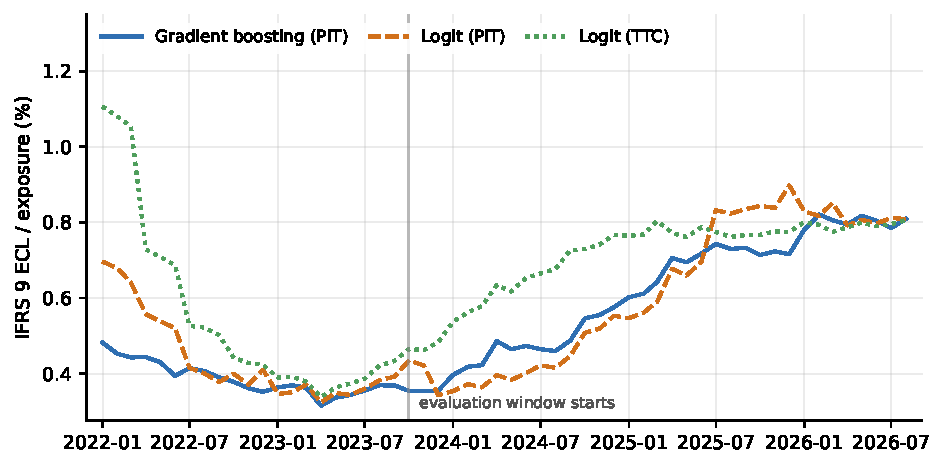
\includegraphics[width=\textwidth]{figures/ecl_paths.pdf}
  \caption{IFRS 9 provisions as a share of exposure, by probability-of-default model. The vertical line marks the
  start of the evaluation window chosen by the training-data rule.}
  \label{fig:paths}
\end{figure}

\begin{table}[t]\centering
  \caption{Amplitude and timing of IFRS 9 provisions over the evaluation window (October 2023 to August 2026).
  Relative rise is the trough-to-peak change divided by the trough, so a constant difference in the level of
  probabilities does not affect it. Leads are the horizon at which the correlation between monthly changes in
  provisions and in the realised stress series is highest; negative means provisions move first.}
  \label{tab:amplitude}
  \begin{tabular}{lrrrrr}
\toprule
& Trough & Peak & Relative & \multicolumn{2}{c}{Lead (months) vs} \\
\cmidrule(lr){5-6}
Model & (\% exp.) & (\% exp.) & rise & new 90+ & new SS \\
\midrule
Gradient boosting (PIT) & 0.35 & 0.82 & $+1.32$ & $-10$ & $0$ \\
Logit (PIT) & 0.34 & 0.90 & $+1.62$ & $-8$ & $-6$ \\
Logit (TTC) & 0.46 & 0.81 & $+0.75$ & $+7$ & $0$ \\
\addlinespace
\midrule
\multicolumn{6}{l}{\emph{Paired differences in relative rise, deal-clustered bootstrap}} \\
\addlinespace[2pt]
\multicolumn{4}{l}{Gradient boosting (PIT) $-$ Logit (PIT)} & \multicolumn{2}{r}{$-0.26$\;$[-0.44,\,-0.09]$} \\
\multicolumn{4}{l}{Gradient boosting (PIT) $-$ Logit (TTC)} & \multicolumn{2}{r}{$+0.59$\;$[+0.35,\,+0.90]$} \\
\multicolumn{4}{l}{Logit (PIT) $-$ Logit (TTC)} & \multicolumn{2}{r}{$+0.85$\;$[+0.56,\,+1.20]$} \\
\bottomrule
\end{tabular}

\end{table}

Table~\ref{tab:amplitude} contains the main result. Provisions built on the PIT logit rise by 1.62 times their
trough level; those built on gradient boosting rise by 1.32; the TTC logit rises by 0.75. The paired difference
between the two point-in-time arms is $-0.26$, with an interval that excludes zero: given the same information,
the machine learning model produced the \emph{less} cyclical provision. The difference between the two logits,
which isolates macro conditioning, is $+0.85$.

Figure~\ref{fig:leadlag} shows the timing counterpart. The point-in-time arms lead newly delinquent balances by
eight to ten months; the through-the-cycle logit does not lead. Realised charge-offs, the series a reader might
expect us to use, are too lumpy at this portfolio size to identify timing, and we report them only for comparison.

\begin{figure}[t]\centering
  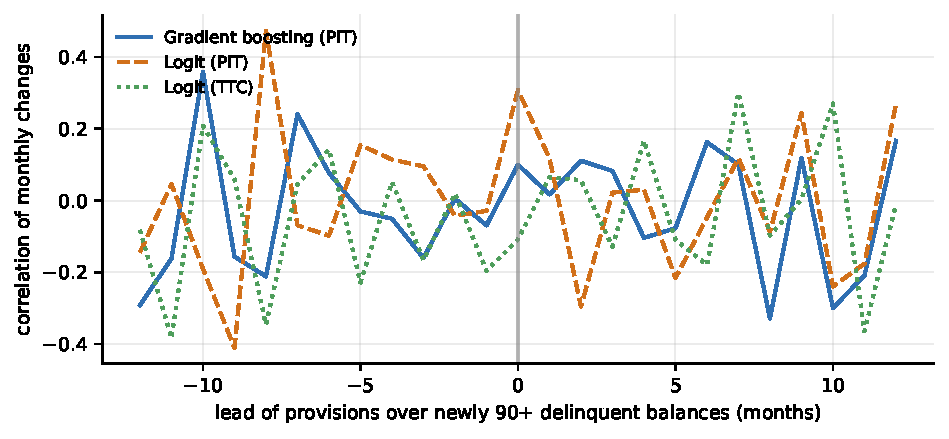
\includegraphics[width=\textwidth]{figures/lead_lag.pdf}
  \caption{Correlation between monthly changes in provisions and in newly 90+ delinquent balances, by lead.}
  \label{fig:leadlag}
\end{figure}

\paragraph{Where the swing comes from.} Decomposing the trough-to-peak change into stage migration and movement
within stages, migration accounts for 43 to 81 per cent of the change depending on the arm and on the order of the
decomposition. The cliff is a feature of the staging architecture, not of any particular model class. Gradient
boosting holds a much larger share of exposure in Stage 2 throughout, averaging 17 per cent within the window
against 6 per cent for the logits (Figure~\ref{fig:stage2}), yet this shows up as a higher level rather than a
larger swing.

\begin{figure}[t]\centering
  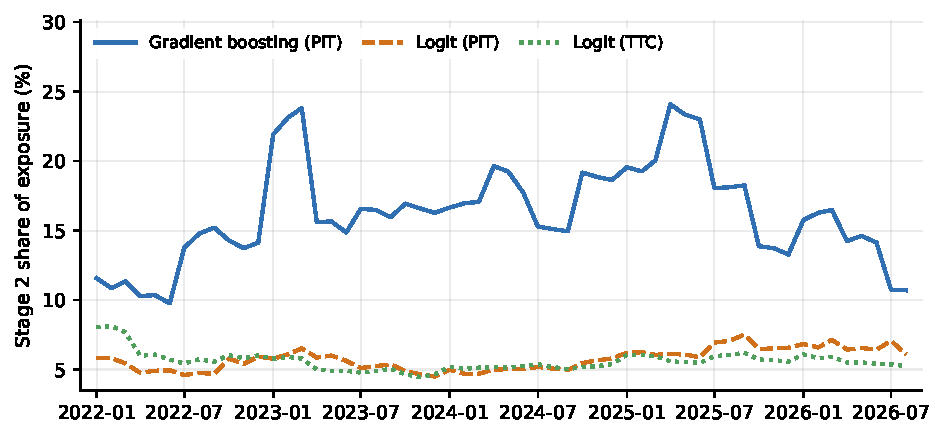
\includegraphics[width=\textwidth]{figures/stage2_share.pdf}
  \caption{Share of exposure in Stage 2.}
  \label{fig:stage2}
\end{figure}

\paragraph{Why the flexible model is less cyclical.} IFRS 9 asks for a probability-weighted view rather than a
single macroeconomic path, so we re-score every arm at each forecast date under a stylised downside (unemployment
1.5 points higher, commercial property prices 10 points lower year on year, credit spreads 100 basis points wider,
with matching state-level shifts) and a milder upside, and weight the resulting provisions 0.5, 0.3 and 0.2.

Two things follow. First, weighting changes almost nothing: the paired difference between the point-in-time arms
becomes $-0.29$ $[-0.46, -0.12]$ against $-0.26$ $[-0.44, -0.09]$ on the single path, and Stage 2 shares move by
less than a tenth of a percentage point. The result does not depend on the single-path simplification.

Second, and more informative, the scenarios expose the mechanism (Table~\ref{tab:sensitivity}). Given the same
macroeconomic inputs and the same shock, the point-in-time logit's mean 12-month probability of default rises by
19.6 per cent in the downside and falls by 16.3 per cent in the upside. The gradient boosting arm barely moves:
0.6 per cent up and 3.2 per cent down. The through-the-cycle logit does not move at all, which is correct by
construction since it has no macroeconomic inputs.

\begin{table}[b]\centering
  \caption{Mean 12-month probability of default under stylised macroeconomic scenarios, evaluation window.}
  \label{tab:sensitivity}
  \begin{tabular}{lrrrrr}
\toprule
& Base & \multicolumn{2}{c}{Downside} & \multicolumn{2}{c}{Upside} \\
\cmidrule(lr){3-4}\cmidrule(lr){5-6}
Model & PD (\%) & PD (\%) & ratio & PD (\%) & ratio \\
\midrule
Gradient boosting (PIT) & 1.43 & 1.44 & 1.006 & 1.39 & 0.968 \\
Logit (PIT) & 1.81 & 2.17 & 1.196 & 1.52 & 0.837 \\
Logit (TTC) & 2.42 & 2.42 & 1.000 & 2.42 & 1.000 \\
\bottomrule
\end{tabular}

\end{table}

This is the result restated at the level of the model rather than the provision. Boosted trees partition on the
features that separate loans, and in this portfolio those are loan-level: leverage, coverage, occupancy,
delinquency. Macroeconomic variables enter with few effectively independent observations, because a decade
supplies only a handful of distinct cyclical states however many loans are observed, and a piecewise-constant
predictor can leave a moderate shift entirely inside the same leaf. A logit has no such freedom: it is told the
relationship is monotone in the macro inputs and extrapolates a response from the same thin time-series variation.
The flexible model is not damping the cycle deliberately; it is declining to learn a macroeconomic response that
the linear model is required to assume. Whether that is prudent or negligent depends on whether the assumed
response is right, which one downturn cannot settle.

\paragraph{Are these provisions plausible?} The provisions here are simulated: no bank booked them, and the
loans sit in securitisation trusts rather than on a balance sheet. A minimum test is whether the staging they
produce resembles what banks report on comparable exposures. It does. Supervisory data for euro area significant
institutions put the Stage 2 ratio for commercial real estate portfolios at 17.8 per cent, down 1.74 percentage
points over the year \citep{ecb2025annual}. Within our evaluation window the gradient boosting arm holds 17.0 per
cent of exposure in Stage 2, the point-in-time logit 5.9 per cent and the through-the-cycle logit 5.4 per cent.
The flexible model therefore lands almost exactly on the reported CRE figure, while both logits look low against
it, and all three are in the region of the roughly 9 per cent Stage 2 share reported across all loan types. This
does not validate the level of any arm, since portfolio composition and bank-specific thresholds differ, but it
does rule out the possibility that the staging machinery here produces figures unlike anything in practice.

\section{Robustness}
\label{sec:robustness}

\begin{table}[t]\centering
  \caption{Paired differences in relative amplitude under alternative specifications, with 95 per cent
  deal-clustered bootstrap intervals.}
  \label{tab:robustness}
  \begin{tabular}{lrr}
\toprule
Specification & GB $-$ Logit(PIT) & Logit(PIT) $-$ Logit(TTC) \\
\midrule
Baseline & $-0.26$\;$[-0.44,\,-0.09]$ & $+0.85$\;$[0.56,\,1.20]$ \\
SICR multiple 1.5 & $-0.22$\;$[-0.38,\,-0.05]$ & $+0.88$\;$[0.59,\,1.23]$ \\
SICR multiple 3 & $-0.28$\;$[-0.46,\,-0.09]$ & $+0.84$\;$[0.54,\,1.21]$ \\
PD source recalibrated & $-0.18$\;$[-0.35,\,0.00]$ & $+1.21$\;$[0.88,\,1.61]$ \\
LGD table bound incl.\ open & $-0.40$\;$[-0.64,\,-0.20]$ & $+0.70$\;$[0.45,\,1.02]$ \\
Window start 2022-01-01 & $-0.15$\;$[-0.38,\,0.04]$ & $-0.49$\;$[-0.84,\,-0.14]$ \\
Window start 2022-07-01 & $-0.16$\;$[-0.38,\,0.05]$ & $+0.36$\;$[0.19,\,0.59]$ \\
Window start 2024-04-01 & $-0.53$\;$[-0.70,\,-0.35]$ & $+1.03$\;$[0.75,\,1.35]$ \\
Special-servicer default definition & $-0.67$\;$[-0.86,\,-0.48]$ & $+0.75$\;$[0.51,\,1.02]$ \\
\bottomrule
\end{tabular}

\end{table}

Table~\ref{tab:robustness} varies one design choice at a time. The machine learning result keeps its sign
throughout and its significance in almost every case: at a significant-increase threshold of 1.5 or 3 rather than
2, when loss given default is raised by imputing the 70 per cent of defaults still unresolved, and under the
broader special-servicer default definition, where it is largest at $-0.67$. The one case in which it is
borderline is recalibration of the probabilities to recent out-of-sample performance, where the interval closes
on zero at $-0.18$ $[-0.35, 0.00]$.

Two sensitivities deserve emphasis rather than a footnote. First, the window. On windows starting before the
training-data rule allows, the machine learning difference is an insignificant null and the macro-conditioning
difference reverses, because the through-the-cycle arm is then still unwinding an unstable early-sample peak. The
amplitude statistic is defined relative to a trough, so the window determines which trough is measured; we
therefore report the pre-committed rule as the headline and the earlier windows in full. Second, the estimator
itself contributes no randomness: with early stopping disabled the gradient boosting fit is deterministic given
the data, and across training-sample draws amplitude varies by only $\pm 0.04$ to $0.08$.

\paragraph{Is the machine learning arm simply starved of data?} The obvious objection to a null, or to a
negative, is that the flexible model never had enough data to behave differently. Three diagnostics answer it.

First, a learning curve. Holding the refit date and the out-of-sample year fixed and training on random subsamples
of loans, gradient boosting improves monotonically with sample size while the logit does not
(Table~\ref{tab:learning} and Figure~\ref{fig:learning}). At 15 per cent of the loans it is far worse than the
logit, by 0.075 of AUC; it overtakes at about half the sample; at the full sample it leads by 0.039 and is still
rising. The sample is therefore binding on the machine learning arm, but the arm is not failing: at the size we
actually have, it ranks defaults better than the logit out of sample.

\begin{table}[b]\centering
  \caption{Out-of-sample default AUC by training-sample size, at a fixed refit date and test year.}
  \label{tab:learning}
  \begin{tabular}{rrrrr}
\toprule
Training loans & Training rows & Defaults & GB AUC & Logit AUC \\
\midrule
15\% & 19,312 & 829 & 0.723 & 0.798 \\
30\% & 38,784 & 1,742 & 0.784 & 0.806 \\
50\% & 65,008 & 2,951 & 0.827 & 0.810 \\
75\% & 97,677 & 4,537 & 0.831 & 0.798 \\
100\% & 129,761 & 6,054 & 0.846 & 0.807 \\
\bottomrule
\end{tabular}

\end{table}

\begin{figure}[b]\centering
  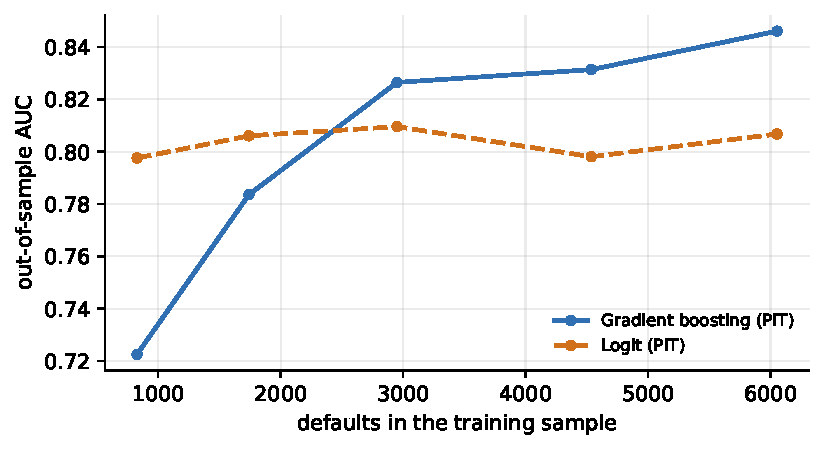
\includegraphics[width=0.8\textwidth]{figures/learning_curve.pdf}
  \caption{Learning curve: out-of-sample AUC against defaults in the training sample.}
  \label{fig:learning}
\end{figure}

Second, if limited data were shrinking the model towards a constant, its predictions would be compressed in every
dimension. They are not. Within the evaluation window the cross-sectional standard deviation of 12-month
probabilities is 0.061 for gradient boosting against 0.056 for the PIT logit, so it separates loans at least as
sharply. What is smaller is its variation over time: the standard deviation of month-on-month changes in the
portfolio mean is 0.17 against 0.29. The arm discriminates as well and moves the aggregate less, which is the
result rather than an artefact of shrinkage.

Third, the estimator contributes no randomness of its own, and re-drawing the training sample moves amplitude by
only $\pm 0.04$ to $0.08$ (Section~\ref{sec:robustness}), well inside the difference being measured.

What this cannot establish is how a machine learning model behaves on a portfolio ten times the size, where its
accuracy advantage would be larger than the 0.04 of AUC seen here. The claim is therefore specific: at this
portfolio size, a measurably more accurate flexible model produced less cyclical provisions.

\section{Discussion}
\label{sec:discussion}
Read against the supervisory concern in Section~\ref{sec:intro}, the results relocate it. The channel the EBA
describes is real, but the part of it that moves provisions is the point-in-time information set, not the
estimator. In our data the flexible model, given exactly that information set, produced a flatter provision path
than the logit. A supervisor reviewing model risk in an IFRS 9 framework and worrying about cyclical amplification
would learn more from the macroeconomic conditioning and the staging rules than from the algorithm class.

That reframing matters because amplitude is not welfare. IFRS 9 exists to correct late recognition, and a
provision that moves earlier is doing what the standard asks of it. Our timing estimates show the point-in-time
arms turning six to ten months ahead of realised delinquency while the through-the-cycle arm does not lead, so the
same conditioning that raises amplitude also delivers timeliness. The policy question is therefore a trade-off
between the two, not a defect to be removed, and it is settled by the choice of information set rather than by the
choice of estimator.

The staging architecture is the other half of the story, and it is common to every arm. Stage migration accounts
for 43 to 81 per cent of the trough-to-peak change in provisions regardless of which model produces the
probabilities. This is the cliff effect anticipated before implementation: a loan that crosses the significant
increase threshold moves from twelve-month to lifetime loss recognition, and in a downturn a large part of a
portfolio crosses at once \citep{esrb2017ifrs9, abad2017cyclical}. Our contribution here is to show that the cliff
is a property of the architecture rather than of any model class: the more flexible model holds two to three times
as much exposure in Stage 2 throughout, yet this raises the level of its provisions rather than the size of their
swing.

\paragraph{External evidence over a genuine crisis.} The sample here contains one downturn, and a natural question
is whether the loss dynamics it implies hold over a severe one. Public loan-level commercial mortgage data covering
2008--2012 exists only for agency multifamily, in Freddie Mac's Multifamily Loan Performance Database \citep{freddie_mlpd}, which
records quarterly status, liquidation balances and realised credit losses for loans funded from 1994. That data is
too thin in defaults to re-estimate the models on: the entire financial crisis produced 90 new defaults on a book
of seven to ten thousand loans, and its covariates are fixed at origination. It is nevertheless informative about
the loss process. Expected loss given default among liquidated multifamily defaults was 33.9 per cent for
liquidations in 2008--2012 against 5.6 per cent for liquidations up to 2007, confirming over a real crisis the
cyclicality that this paper's provisions are built on.

It also isolates where that cyclicality lives. Severity conditional on a loss is close to constant: 45.5 per cent
in the multifamily crisis cohort, 44.8 per cent across the whole multifamily sample since 1994, and 46.2 per cent
among the terminal credit events in our own CMBS sample, with fitted beta densities whose means agree to within
half a percentage point. What moves over the cycle is the probability that a default produces any loss at all,
which runs from about a quarter in benign periods to more than three quarters in the crisis cohort. For
provisioning this matters: the cyclical content of expected credit loss enters through default and through the
probability that default becomes a loss, and much less through how severe losses are when they occur.

\paragraph{Limitations.} The evidence covers one asset class, prime US commercial mortgages, and one downturn, the
commercial real estate deterioration of 2023 to 2026. With 1{,}102 defaults and 173 realised losses, loss given
default is estimated on the portfolio as a whole rather than by segment. The bootstrap resamples deals, so it
reflects cross-sectional uncertainty and not uncertainty about the single macroeconomic episode. We expect no
transfer of the point estimates to corporate or retail portfolios; the mechanism, not the magnitude, is what
should travel. Finally, the accuracy advantage of gradient boosting in this setting is small out of sample, +0.00
to +0.04 in AUC for in-term defaults among performing loans. The learning curve in Section~\ref{sec:results}
shows that gap widening with sample size, so a larger portfolio could give a different answer; this design speaks
to portfolios of this size.

\section{Conclusion}
Holding loss given default, exposure and the staging rules fixed, and giving a machine learning model exactly the
information a logit has, we find no evidence that machine learning makes IFRS 9 provisions more procyclical, and
some evidence that it makes them less so. The amplification that regulators are looking for sits in macroeconomic
conditioning and in stage migration.

\bibliographystyle{chicago}
\bibliography{refs}

\end{document}
